%%\documentclass[handout]{beamer}
\documentclass[]{beamer}
\usetheme[secheader]{Boadilla}

\usepackage{tikz}
\usetikzlibrary{shapes.callouts}

\mode<presentation>{}

\usepackage{boxedminipage}
\usepackage{pgf}
\usepackage{graphicx}
\usepackage{amsmath}
\usepackage{amssymb,amsmath,amsthm}
\usepackage{colortbl}
\usepackage{xspace}
\usepackage{xcolor}

\usepackage{amssymb,amsmath,amsthm}
\usepackage{boxedminipage}

\beamerboxesdeclarecolorscheme{monscheme}{structure}{gray!25}
\beamertemplatetransparentcovereddynamic


\colorlet{myblue}{blue!80!black}
\colorlet{mygreen}{green!80!black}

\newcommand{\from}{\leftarrow}
\newcommand{\ignore}[1]{}
\newcommand{\algofont}[1]{{\mathsf{#1}}}
\newcommand{\gamefont}[1]{{\mathsf{#1}}}
\newcommand{\objfont}[1]{{\mathtt{#1}}}
\newcommand{\secprm}{\lambda}

\newcommand{\calA}{\mathcal{A}}
\newcommand{\calD}{\mathcal{D}}
\newcommand{\calF}{\mathcal{F}}
\newcommand{\st}{\mathtt{st}}


\newcommand{\anamorphicPrefix}{\algofont{a}}
\newcommand{\anamorphicPrefixObj}{\objfont{a}}
\newcommand{\ame}{\algofont{AME}}
\newcommand{\akg}{\anamorphicPrefix\kg} 
\newcommand{\aenc}{\anamorphicPrefix\enc}
\newcommand{\adec}{\anamorphicPrefix\dec}
\newcommand{\apk}{\anamorphicPrefixObj\pk}
\newcommand{\ask}{\anamorphicPrefixObj\sk}
\newcommand{\dkey}{\objfont{dkey}}
\newcommand{\act}{\anamorphicPrefixObj\ct}
\newcommand{\amsg}{\anamorphicPrefixObj\msg}


%%anamorphic games
\newcommand{\RealG}{\gamefont{RealG}}             %real
\newcommand{\AnamorphicG}{\gamefont{AnamorphicG}} %anamorphic 
\newcommand{\Oa}{\algofont{Oa}}
\newcommand{\Oe}{\algofont{Oe}}

%algorithms for encryption schemes
%\newcommand{\encryptionSchemeName}{\calE}
\newcommand{\E}{\algofont{E}}
\newcommand{\kg}{\algofont{KG}}
\newcommand{\enc}{\algofont{Enc}}
\newcommand{\dec}{\algofont{Dec}}
%objects of encryption schemes
\newcommand{\pk}{\objfont{pk}}      %public key
\newcommand{\sk}{\objfont{sk}}      %secret key
\newcommand{\msg}{\objfont{msg}}    %cleartext
\newcommand{\ct}{\objfont{ct}}      %ciphertext

%encryption scheme with pseudoR ciphertexts
\newcommand{\prPrefix}{\algofont{pr}}
\newcommand{\prObjPrefix}{\objfont{pr}}
\newcommand{\prEname}{\prPrefix\E}
\newcommand{\prkg}{\prPrefix\kg}
\newcommand{\prenc}{\prPrefix\enc}
\newcommand{\prdec}{\prPrefix\dec}
\newcommand{\prct}{\prObjPrefix\ct}
\newcommand{\prkey}{\prObjPrefix\objfont{K}}


\newcommand{\rrdec}{\algofont{rr}\dec}


\newcommand{\PameG}{\gamefont{SingleAnG}}        %private anamorphic --> single



\title[Anamorphic Encryption]{The Self-Anti-Censorship Nature of Encryption}
\subtitle{On the Prevalence of Anamorphic Encryption}
%\title[Short Title]{Long Title}
\author{author1 \inst{1} \and author2 \inst{1} \and author3 \inst{2}}


\author[KPPYZ]{M.Kuty{\l}owski\inst{1}, GP\inst{2}, D.H.Phan\inst{3}, M.Yung\inst{4}, M.Zawada\inst{5}}
\institute[]{
\inst{1} Wroc{\l}aw University of Science and Technology, and NASK - National Research Institute 
\and \inst{2} Universit\`a di Salerno and Google
\and \inst{3} Telecom Paris, Institute Polytechnique de Paris
\and \inst{4} Google and Columbia University
\and \inst{5} Wroc{\l}aw University of Science and Technology 
}

\date{}

\begin{document}

\begin{frame}
  \titlepage


PETS 2023 -- Lausanne
\end{frame}


\begin{frame}
\frametitle{Privacy as a Human Right}

UDHR, Article 12: (1948)

{\color{brown}
{\em No one shall be subjected to arbitrary interference with his privacy, family, home or correspondence,...}
}

\pause
\vskip 1cm
\begin{block}{End to End Encryption}
\begin{itemize}
\item Cryptography has been very successful in providing tools for
encrypting communication
\begin{itemize}
\item The Signal protocol and app \hfill \includegraphics[width=.5cm]{imgs/signal}
\end{itemize}
\end{itemize}
\end{block}

\pause
\vfill
But its success relies on an 
{\color{red} assumption} that might be challenged in dictatorial
states
\end{frame}

\begin{frame}
\frametitle{The receiver-privacy assumption}

{\color{brown} \em 
Encryption guarantees message confidentiality only with respect to 
parties that do not have access to  the receiver's private key
}

\vfill


\begin{block}{The receiver-privacy assumption}
The receiver keeps his secret key in a private location
\end{block}

\end{frame}

\begin{frame}
\frametitle{Ok...one more assumption}

Why is this a problem?

\begin{theorem}
Assume 
{\color{brown} existence of one-way functions} 
and 
{\color{brown} receiver privacy}.
Then, there exist secure symmetric encryption schemes.
\end{theorem}

\vfill
\begin{block}{Two assumptions}
\begin{itemize}
\item Existence of one-way functions
\item Ability to protect my key
\end{itemize}
\end{block}
\end{frame}

\begin{frame}
\frametitle{Law of Nature vs Normative Prescription}

\begin{itemize}
\item {\color{mygreen} Assumption of the existence of one-way functions comes from
{\em our current scientific understanding of Nature}}
 
    \begin{itemize}
        \item {\color{blue}if true, it is enforced by Nature}
        \item {\color{blue}it might be false but then it is false for all}
    \end{itemize}
\vskip 1cm
\item {\color{mygreen} Receiver privacy is a {\em norm}: }
    
    \begin{itemize}
        \item {\color{blue} it is enforced by political power}
        \item {\color{blue} it can be changed by law, decree, force}
        \item {\color{blue} it could change for some but not for all}
    \end{itemize}
\end{itemize}

\end{frame}

\begin{frame}
\frametitle{Receiver privacy}
\begin{itemize}
\item Realistic for ``{\color{purple} normal}'' settings
\item No wonder that encryption has been developed under this assumption
\begin{itemize}
\item with no explicit mention
\end{itemize}
\vskip .5cm
\item In a dictatorship, instead
\begin{itemize}
\item {\color{blue} No receiver privacy:} 
citizens might be {\color{red} ``invited''} to surrender their private keys

\centerline{\includegraphics[width=4.5cm]{imgs/xkcd}}
\vfill
\hfill thanks to {\tt https://xkcd.com/538/}

\end{itemize}
\end{itemize}
\end{frame}


\begin{frame}
\frametitle{Not only dictators...}
\begin{block}{The Clipper Chip}
{\em\color{brown} Presently, anyone can obtain encryption devices for voice or data transmissions[...]
if criminals can use advanced encryption technology in
their transmissions, electronic surveillance techniques could be rendered 
useless because of law enforcement’s inability to decode the message.}

\hfill {\color{teal} Howard S. Dakoff}

\hfill {\color{teal} {\em The Clipper Chip Proposal}}

\hfill {\color{teal} J. Marshall L. Rev., 29, 1996.}
\end{block}

\begin{block}{Ban of E2E encryption}
\color{brown}{\em
In our country, do we want to allow a means of communication between people which even in extremis, with a signed warrant from the Home Secretary personally, that we cannot read?}

\color{teal}
\hfill David Cameron

\hfill UK Prime Minister

\hfill January 2015
%%https://www.bbc.com/news/technology-33737813
\end{block}
\end{frame}

\begin{frame}
\frametitle{How can we fix this?}

{\color{blue} Not by designing new schemes}

\pause

\begin{itemize}
\item Suppose we design an encryption scheme that is secure 
without assuming receiver privacy 

\item What is the dictator going to do?

    \begin{itemize}
    \item It will be considered illegal
    \item The simple act of using the new scheme will be self accusatory
    \item The encryption scheme and its use will be seen as provocations
    \end{itemize}

\end{itemize}

\pause

\vskip 1cm
{\color{brown}\em 
Rather, we should look at {\em existing} schemes to see if they can
be used to defeat the dictator
}

\pause

\vfill
Existing schemes cannot be disallowed as there are legitimate uses for
them. Legitimate, even for the dictator.
\end{frame}

\begin{frame}
\frametitle{Anamorphic Encryption [PPY -- Eurocrypt 2022]}

\begin{block}{The anamorphic approach [P-Phan-Yung Eurocrypt '22]}
\begin{itemize}
\item {\color{green} one} public key $\color{blue} \pk$, 
    {\color{green} one} ciphertext,
    {\color{green} one} secret key $\color{blue} \sk$
    \begin{itemize}
        \item \color{brown} that's what the dictator thinks
    \end{itemize}
\pause
\item {\color{green} one} public key $\color{blue} \pk$,
{\color{green} one} ciphertext,
{\color{purple} two} secret keys $\color{blue} \sk,\dkey$, 
    \begin{itemize}
        \item {\color{green} one} ciphertext, {\color{purple} two}
            plaintexts $\color{blue} \msg,\amsg$
    \end{itemize}
\end{itemize}
\end{block}
%%The same ciphertext reveals different plaintexts depending on how you look at it
\pause

\only<4>{\centerline{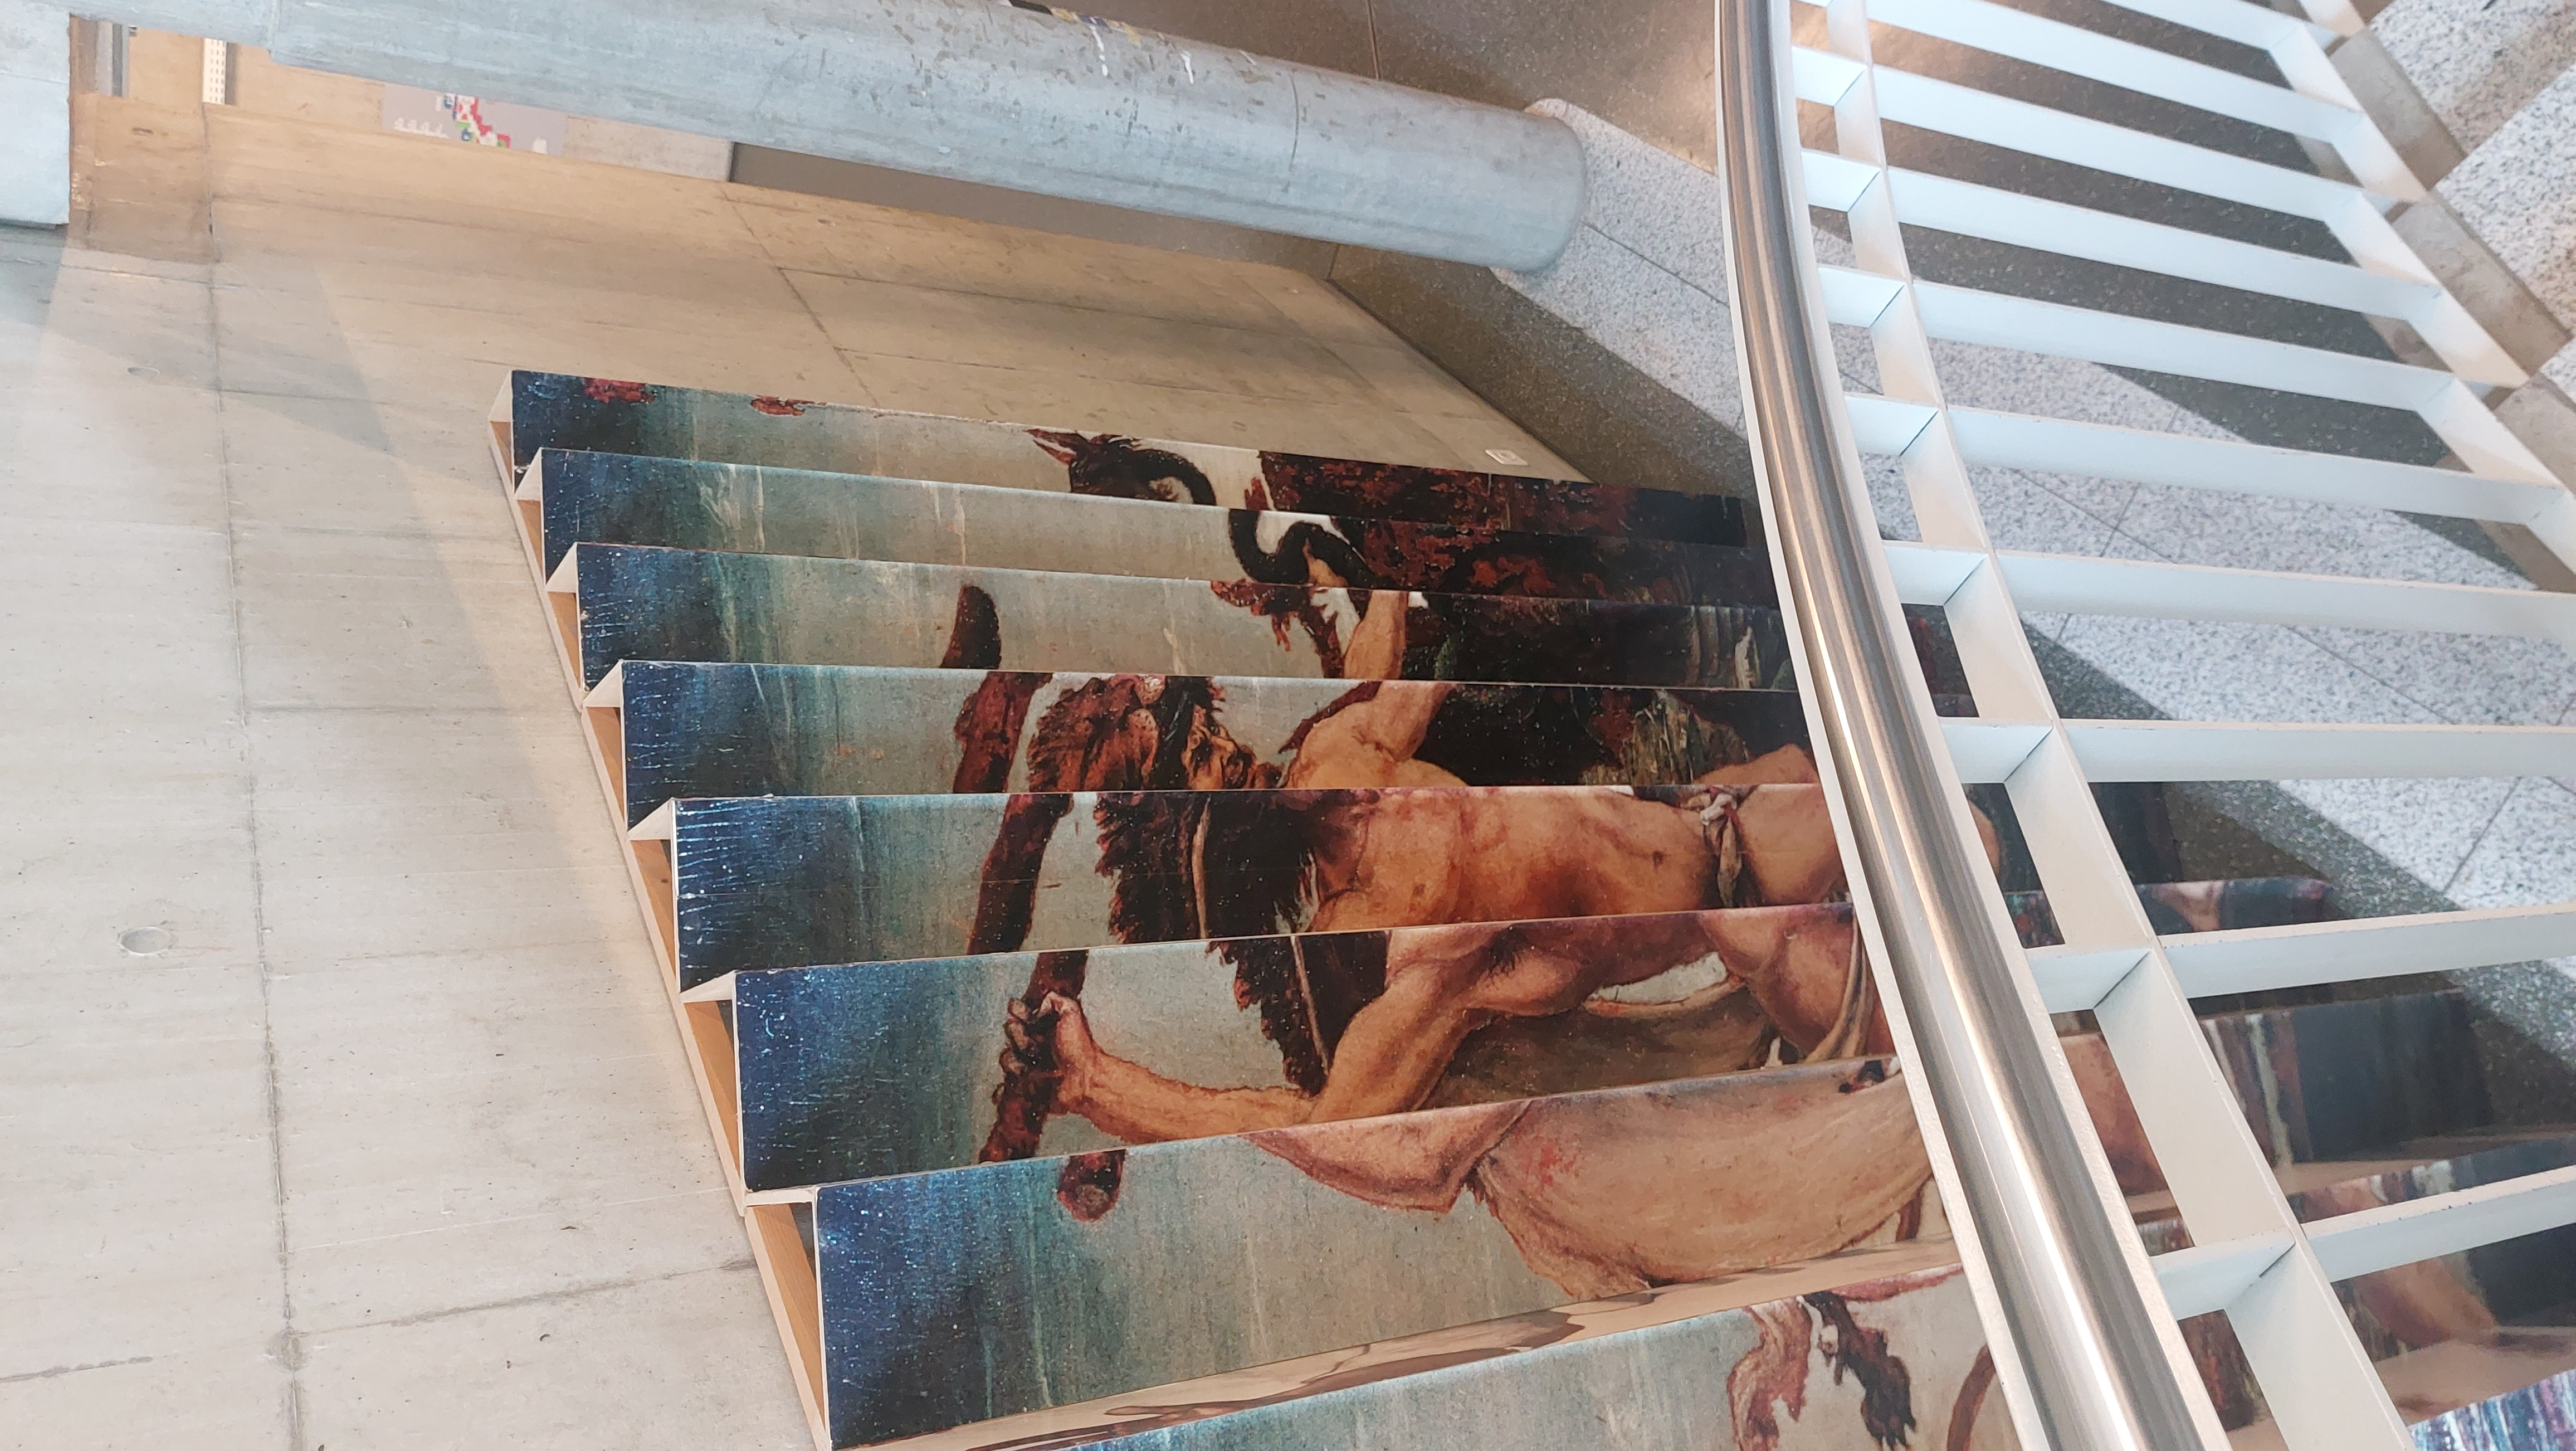
\includegraphics[width=4cm,angle=270]{imgs/anam1.jpg}}}
\only<5>{\begin{center}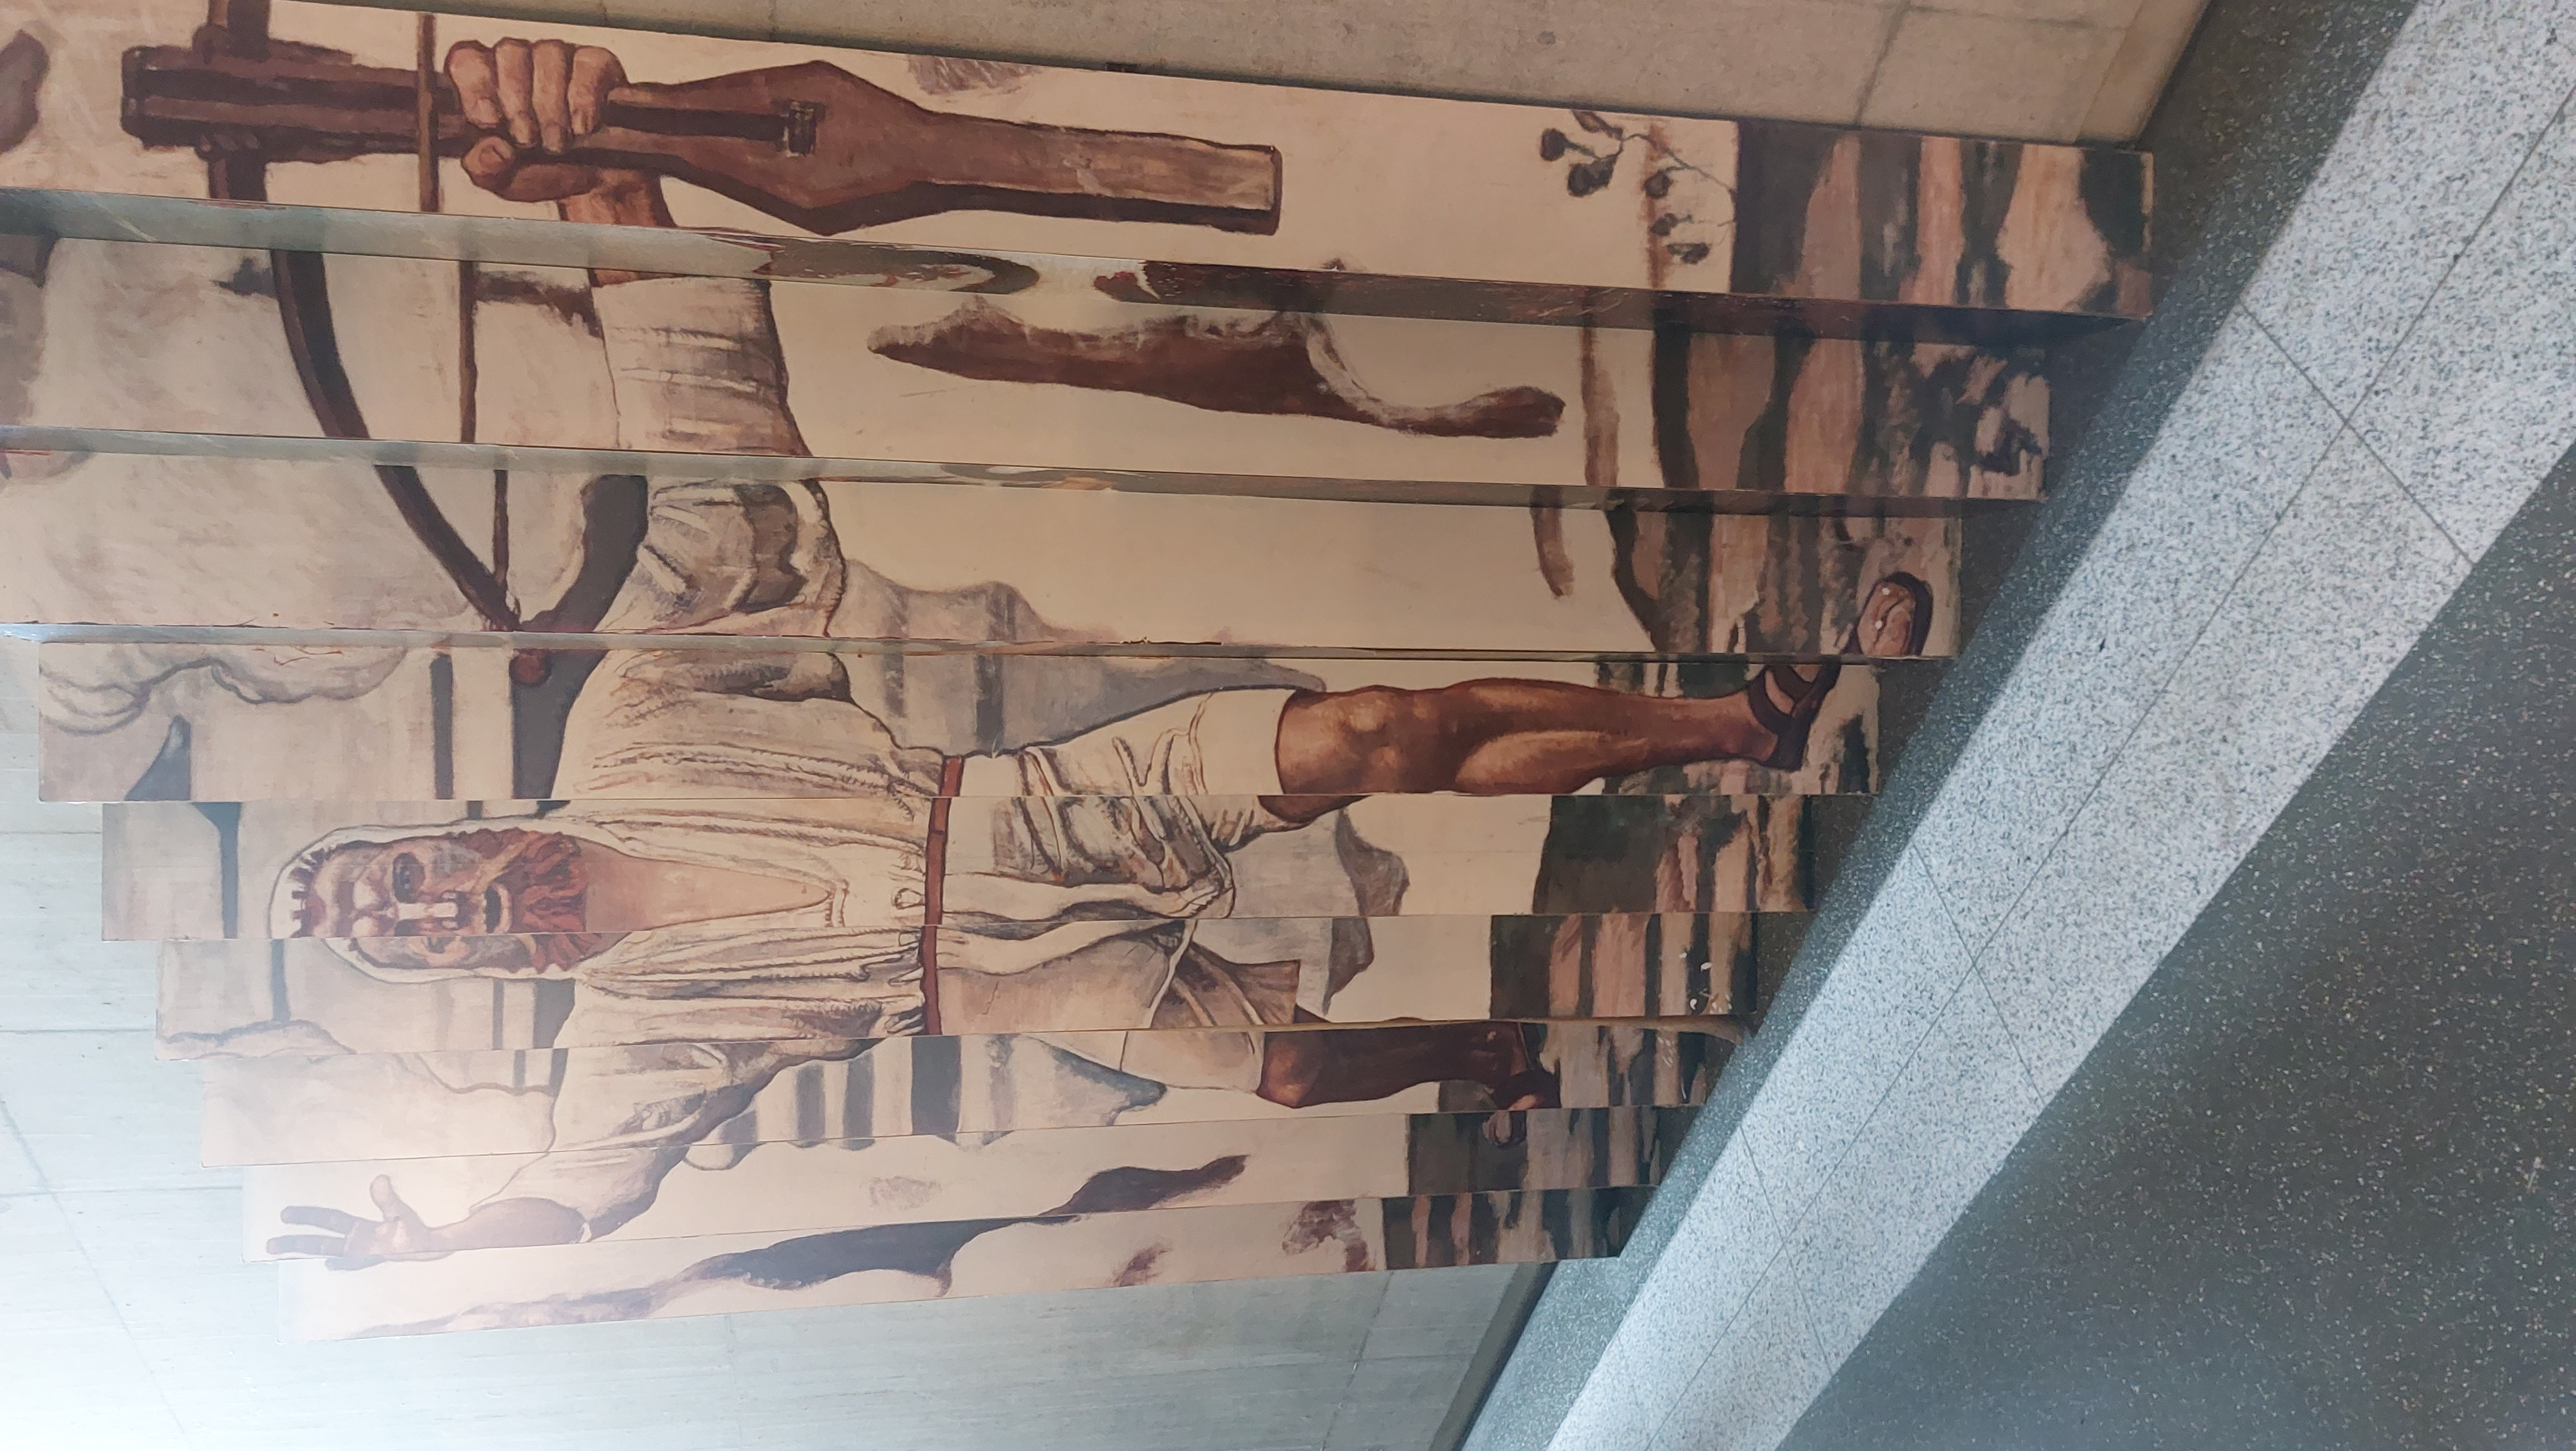
\includegraphics[width=4cm,angle=270]{imgs/anam2.jpg}\end{center}}
\end{frame}

\begin{frame}

\frametitle{Previous work}
\begin{block}{P-Phan-Yung [Eurocrypt '22]}
\begin{itemize}
\item every scheme can be made anamorphic with low rate
    \begin{itemize}
        \item $\color{blue}\amsg$ of length {\em\color{purple}logarithmic}
    in $\secprm$
    \end{itemize}
\item Naor-Yung encryption scheme is anamorphic
    \begin{itemize}
        \item $\color{blue}\amsg$ of length {\em\color{purple}polynomial}
        in $\secprm$
    \end{itemize}
\end{itemize}
\end{block}


\end{frame}

\begin{frame}
\frametitle{Contributions of this paper}

\begin{block}{Contributions}
\begin{itemize}
\item present refined notion
    \begin{itemize}
        \item {\color{purple} Single-Receiver} anamorphic encryption
        \item {\color{purple} Multi-Receiver} anamorphic encryption
    \end{itemize}
\item give evidence of the {\em\color{purple} prevalence} of
anamorphic encryption
            \begin{itemize}
                \item RSA-OAEP, Goldwasser-Micali, Paillier, ElGamal, Cramer-Shoup, Smooth Projective Hash Function are efficiently anamorphic 
            \end{itemize}
\end{itemize}
\end{block}
\pause
\vfill
\begin{block}{This talk}

\begin{itemize}

\item RSA-OAEP is anamorphic
\item Single- vs Multi-Receiver anamorphic
\item RSA-OAEP is Multi-Receiver anamorphic
\end{itemize}

\end{block}
\end{frame}

\begin{frame}
\begin{block}{In concrete terms}

An encryption scheme $\color{brown}\E=(\kg,\enc,\dec)$ is {\color{red}\em anamorphic}
if it admits an {\color{blue}\em anamorphic triplet $(\akg,\aenc,\adec)$}
that is 
{\color{blue}\em indistinguishable} from $\E$ to the eyes of
the {\color{red} dictator $\calD$} (that has the secret key).

\end{block}
\end{frame}

\begin{frame}
\frametitle{RSA-OAEP: an example}

To show that 
{\color{brown} RSA-OAEP}$\color{brown}=(\kg,\enc,\dec)$ is {\color{red} anamorphic},
we design an {\color{blue}\em anamorphic triplet $(\akg,\aenc,\adec)$}

\vfill

\begin{itemize}
\item $\color{blue} \akg$ outputs one public key $\color{blue} \apk$, and two secret keys $\color{blue} \ask$ and $\color{blue} \dkey$
\item $\color{blue} \aenc$ takes two messages, regular $\color{blue} \msg$ and {\em \color{blue} anamorphic $\amsg$}, 
and outputs one ciphertext $\color{blue} \act$
\item $\color{blue} \dec$ on input $\color{blue} \act$ and $\color{blue} \ask$ outputs $\color{blue} \msg$
\item $\color{blue} \adec$ on input $\color{blue} \act$ and $\color{blue} \dkey$ outputs $\color{blue} \amsg$

\vskip 1cm
\item share $\color{blue}\dkey$ with your intended recipients
\item you pretend to be using 
{\color{blue} RSA-OAEP} and, when asked, you surrend $\color{blue} \ask$

\item the dictator $\calD$ cannot tell if you are using
$\color{blue}(\akg,\aenc,\adec)$
or
$\color{brown}\text{RSA-OAEP}=(\kg,\enc,\dec)$

\end{itemize}

\end{frame}

\begin{frame}
\frametitle{Anamorphic Triplet}

$\color{brown} (\akg,\aenc,\adec)$

\begin{itemize}
    \item {\color{blue} {\em anamorphic key generation} $\akg$ }
        \begin{itemize}
            \item input: the security parameter $1^\secprm$
            \item output: $(\apk,\ask)$ pair of keys and
            {\color{purple} {\em double} key $\dkey$};
        \end{itemize}
\vfill
\item 
{\color{blue} {\em anamorphic encryption} $\aenc$}
        \begin{itemize}
            \item input:

            {\color{teal} two keys:}
        public key $\apk$ and {\color{purple} {\em double key} $\dkey$}, and

            {\color{teal} two messages:} {\em regular message} $\msg$, and
            {\color{purple} {\em anamorphic message} $\amsg$}

            \item output: {\color{teal} one ciphertext} $\act$;
        \end{itemize}
\vfill
\item 
{\color{blue} {\em anamorphic decryption} algorithm $\adec$}
        \begin{itemize}
            \item input: 

            {\color{teal} two keys:} $\ask,\dkey$ 

            {\color{teal} one ciphertext:} $\act$;
         \item output: message $\msg$;
        \end{itemize}
\end{itemize}
\end{frame}

\begin{frame}


\begin{center}
\begin{boxedminipage}[t]{12cm}
$\color{brown} \RealG_{\E,\calD}(\secprm)$
\begin{enumerate}
\item Set $\color{brown} (\pk,\sk)\from\kg(1^\secprm)$
\item Return $\color{brown} \calD^{\Oe(\pk,\cdot,\cdot)}(\pk,\sk)$,
where
\\
$\color{brown} \Oe(\pk,\msg,\amsg)=\enc(\pk,\msg).$
\end{enumerate}
\end{boxedminipage}
\vfill
\begin{boxedminipage}[t]{12cm}
$\color{blue} \AnamorphicG_{\ame,\calD}(\secprm)$
\begin{enumerate}
\item Set $\color{blue} ((\apk,\ask),\dkey)\from\akg(1^\secprm)$
\item Return $\color{blue} \calD^{\Oa(\apk,\dkey,\cdot,\cdot)}(\apk,\ask)$,
where\\
$\color{blue} \Oa(\pk,\dkey,\msg,\amsg)=\aenc(\apk,\dkey,\msg,\amsg).$
\end{enumerate}
\end{boxedminipage}
\end{center}
\end{frame}

                           
\begin{frame}
\frametitle{A general strategy for proving anamorphism}

\begin{itemize}
\item IND-CPA $\color{brown} \E=(\kg,\enc,\dec)$ must be randomized
\item Some encryption schemes allow to extract the randomness used
to produce the ciphertext by running $\color{brown} \rrdec$
    \begin{itemize}
        \item $\color{brown}\rrdec(\enc(\pk,\msg;R),\sk)\rightarrow(R,\msg)$
    \end{itemize}
\item Replace the randomness with the ciphertext of an encryption scheme
$\color{brown} \prEname=(\prkg,\prenc,\prdec)$ with pseudo-random ciphertexts
\end{itemize}

\vfill

\color{teal}
Pseudo-random ciphertexts from one-way functions

AES ciphertexts are conjectured to be pseudo-random
\end{frame}

\begin{frame}

\frametitle{The anamorphic triplet}

\begin{exampleblock}{Anamorphic key generation $\akg(1^\secprm)$}
\begin{itemize}
    \item compute $\color{brown}(\apk,\ask)\from\kg(1^\secprm)$;
    \item compute $\color{blue}\prkey\from\prkg(1^\secprm)$;
    \item set $\color{blue}\dkey=(\prkey,\ask)$;
\end{itemize}
\end{exampleblock}

\begin{exampleblock}{Anamorphic encryption $\aenc(\apk,\dkey,\msg,\amsg)$}
\begin{itemize}
    \item compute $\color{blue} R\from\prenc(\dkey,\amsg)$
    \item compute $\color{brown} \act\from\enc(\apk,\msg;R)$
\end{itemize}
\end{exampleblock}

\begin{exampleblock}{Anamorphic decryption $\adec(\ask,\dkey,\act)$}
\begin{itemize}
    \item compute $\color{brown} (R,\msg)\from\dec(\ask,\act)$
    \item compute $\color{blue} \amsg\from\prdec(R,\dkey)$
\end{itemize}
\end{exampleblock}
\end{frame}

\begin{frame}
\frametitle{RSA-OAEP is Anamorphic}

\begin{block}{RSA-OAEP encryption}
To encrypt $\msg$ of length $n/2$ with hash functions $G$ and $H$
\begin{itemize}
    \item randomly select $\color{brown} R\from\{0,1\}^n$
    \item set $\color{brown} M=\msg||0^{n/2}$
    \item set $\color{brown} \hat M=G(R)\oplus M$
    \item set $\color{brown} P=\hat M||(R\oplus(H(\hat M)))$
    \item encrypt $\color{brown} P$ using RSA
\end{itemize}

\vskip 1cm
To recover $\color{brown} R$ from $\color{brown} P$,
just XOR the hash of the left half and the right half of $\color{brown} P$.

\end{block}
\end{frame}

\begin{frame}
\frametitle{Multi- vs Single-Receiver}
\begin{itemize}
\item $\color{blue} \dkey$ for RSA-OAEP contains $\color{blue} \ask$
\item necessary to extract randomness
\item one obtains both $\color{blue} \msg$ and $\color{blue} \amsg$ 
\item $\color{blue} \msg$ (and $\color{blue} \amsg$) is
{\color{teal}\em multi-receiver}:
every user with $\color{blue}\dkey$ can read it.
\end{itemize}
\end{frame}

\begin{frame}
\frametitle{Single-Receiver Anamorphic}
IND-CPA holds also for users that have $\dkey$

\begin{center}
\begin{block}{Game for Single-Receiver Anamorphism}
\color{brown}
$\PameG_{\ame,\calA}^\beta(\secprm)$
\begin{itemize}
\color{brown}
\item Set $((\apk,\ask),\dkey)\from\akg(1^\secprm)$
\item $(\msg_0,\msg_1,\amsg,\st)\from\calA(\apk,\dkey)$;
\item $\act\from{\Oe^\beta(\apk,\dkey,\msg_0,\msg_1,\amsg)}$;
\item return $\calA(\act,\st)$,
where
\\
$\Oe^\beta(\apk,\dkey,\msg_0,\msg_1,\amsg)=\aenc(\apk,\dkey,\msg_\beta,\amsg).$
\end{itemize}
\end{block}
\end{center}

\begin{theorem}
Cramer-Shoup is single-receiver anamorphic
\end{theorem}
\end{frame}
\begin{frame}
\frametitle{Conclusion}

\vfill
{\em \color{teal}
anamorphic encryption is fairly practical and implementable with many 
standard schemes for anamorphic messages  of a few hundred of bits }

\vfill

\end{frame}

\begin{frame}
\frametitle{Related ePrint reports}
\begin{itemize}
\item Extended version of this paper:

{\color{teal}
Mirek Kutylowski, Giuseppe Persiano, Duong Hieu Phan, Moti Yung, Marcin Zawada:
{\em The Self-Anti-Censorship Nature of Encryption: On the Prevalence of Anamorphic Cryptography.} IACR Cryptol. ePrint Arch. 2023: 434 (2023)
}

\item Original paper from Eurocrypt 2022:

{\color{teal}
	Giuseppe Persiano, Duong Hieu Phan, Moti Yung:
{\em Anamorphic Encryption: Private Communication against a Dictator.} IACR Cryptol. ePrint Arch. 2022: 639 (2022)
}

\item Upcoming paper on anamorphic signatures from CRYPTO 2023:

{\color{teal}
	Mirek Kutylowski, Giuseppe Persiano, Duong Hieu Phan, Moti Yung, Marcin Zawada:
{\em Anamorphic Signatures: Secrecy From a Dictator Who Only Permits Authentication!} IACR Cryptol. ePrint Arch. 2023: 356 (2023)
}

\end{itemize}
\end{frame}

\end{document}

